\documentclass{../mcstext}

\texttitle{Лекция 4:  Моделирование и анализ}

\begin{document}

\maketitle
\thispagestyle{empty}

\section{Введение}

В этой лекции речь пойдёт не про UML (точнее, не только про UML), а про использование моделирования в фазе анализа предметной области. Анализ требований, анализ предметной области --- самые первые и самые важные этапы проекта, поэтому и моделирование на этих этапах применяется очень активно, даже теми, кто ненавидит UML всей душой. Существует довольно много разных визуальных языков, краткий обзор их и будет в этой лекции.

\section{Моделирование требований}

Первый этап жизненного цикла любого программного продукта --- это сбор и анализ требований, и уже на этом этапе применяются техники, связанные с визуальными языками. Для чего вообще нужно формализовывать требования:

\begin{itemize}
    \item Прежде всего для того, чтобы понимать, что мы хотим сделать. Требования нужны самим разработчикам (есть известная поговорка <<Без хорошего ТЗ получается... не очень>>).
    \item Формализованные требования --- это своего рода соглашение между разработчиками, заказчиками и пользователями. Обратите внимание, что заказчики и пользователи часто не одно и то же лицо, и требования у них могут быть разными. Например, при разработке компьютерной игры заказчиком выступает издатель и его цель --- заработать как можно больше денег, а пользователями выступают, например, ленивые школьники, цель которых --- весело провести время. Фиксация требований позволит их, во-первых, оценить на предмет соответствия ожиданиям всех участников процесса, во-вторых, обсудить со всеми участниками, чтобы потом ни к кому ни у кого не было претензий.
    \item Требования --- это чёткое обозначение границ системы: что мы хотим делать, а что точно не хотим. Это позволяет противостоять feature creep-у, эффекту постепенного появления новых требований в процессе разработки, который может сильно затянуть или даже сорвать проект.
    \item Требования --- это входные данные для следующей фазы жизненного цикла, планирования проекта.
\end{itemize}

Чаще всего требования описываются словесно, неформально или полуформально (например, через <<user story>> в Scrum и других Agile-методологиях). Есть полуформальные визуальные языки описания требований (например, диаграмма случаев использования UML, но она требует и текстовых описаний тоже), есть более-менее формальные модели, например, диаграмма требований SysML.

\subsection{Диаграмма случаев использования UML}

Первый визуальный язык, используемый для анализа требований (он же самый популярный), который мы рассмотрим --- диаграммы случаев использования UML (также известные как диаграммы прецедентов, use case-диаграммы). Они появились до UML, как часть методологии OOSE, разработанной Айваром Якобсоном в 1992 году. OOSE на самом деле строилась вокруг случаев использования, их предлагалось продумать первыми, затем на их базе уже проектировать остальную архитектуру, непрерывно поддерживая связь со случаями использования (чтобы не делать лишней работы и быть уверенными, что вся требуемая функциональность где-то реализована). Потом Якобсон перешёл на работу в Rational и стал одним из трёх основателей UML, диаграммы случаев использования попали в язык практически без изменений.

Диаграммы очень простые, состоят всего из двух типов сущностей и границы системы:

\begin{center}
    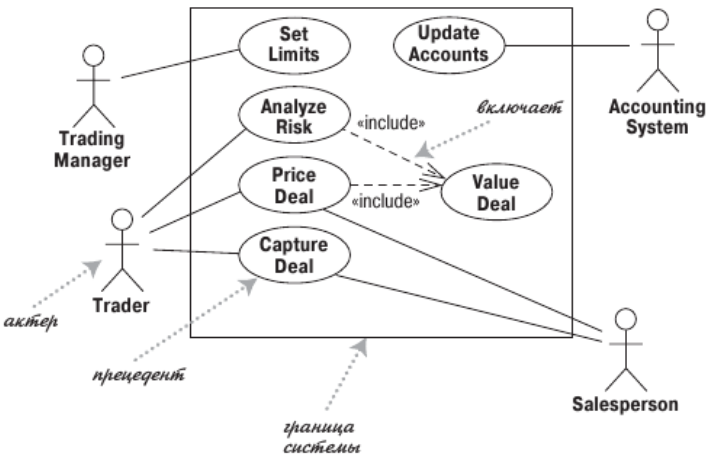
\includegraphics[width=0.6\textwidth]{useCaseDiagram.png}
    \attribution{М. Фаулер, UML. Основы}
\end{center}

\begin{itemize}
    \item Акторы (или актёры, роли, это всё неудачные переводы со шведского на английский и с английского на русский) --- внешние сущности, использующие систему. Это могут быть группы пользователей, объединённые общей целью использования системы (роли, собственно). Это могут быть также внешние программные системы, которые пользуются нашей. Иногда в качестве акторов рисуются и другие программные системы (или люди), которые нужны нашей системе для работы, но это неканонично и лучше так не делать, чтобы не путать читателей.
    \item Случаи использования (прецеденты)  --- цель использования системы актором. Это одно-два-три слова, описывающие, что пользователь хочет в итоге получить (например, <<Проанализировать риски>>, <<Оценить сделку>>). Их часто путают с функциональностью системы, например, <<Залогиниться>> --- это не то же самое. Пользователь никогда не имеет целью использования системы залогиниться, в лучшем случае он хочет безопасного выполнения всех операций, но нефункциональные требования --- это тоже не случаи использования, так что на этой диаграмме не рисуются.

    Случаи использования формулируются слишком кратко, чтобы быть полезными сами по себе, поэтому каждый случай использования должен раскрываться в один или несколько \textit{сценариев использования} системы. Сценарии использования как раз и говорят, что и в каком порядке делает пользователь, чтобы достичь цели (например, логинится -> выбирает нужную сделку -> анализирует риски -> описывает результаты анализа в соответствующую форму). Сценарии чаще всего описываются просто текстом, часто неформальным, иногда как-то структурированным (например, user story из Scrum). Если вы очень любите визуальное моделирование, сценарии использования можно описывать диаграммами активностей UML.
\end{itemize}

Случаи использования на диаграмме могут быть связаны отношениями, позволяющими их структурировать. Например, отношение Include:

\begin{center}
    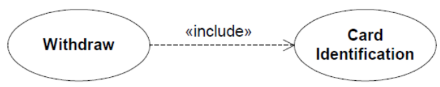
\includegraphics[width=0.45\textwidth]{useCaseInclude.png}
    \attribution{OMG, UML 2.5 Specification}
\end{center}

Include означает, что один случай использования включает в себя другой, например, при снятии налички пользователь хочет, чтобы система идентифицировала его банковскую карту (вряд ли пользователь может отдельно хотеть именно этого, так что пример не очень каноничен, зато из стандарта языка).

Отношение Extend:
\begin{center}
    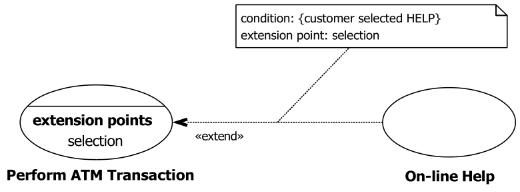
\includegraphics[width=0.5\textwidth]{useCaseExtend.png}
    \attribution{OMG, UML 2.5 Specification}
\end{center}

Это отношение означает, что один случай использования имеет одну или несколько точек расширения, в которых может использоваться функциональность, связанная с другим случаем использования. Например, <<Проведение транзакции с помощью банкомата>> имеет точки расширения, где пользователь может получить справку по использованию системы. Это может выражаться в связанных сценариях использования, например, словами <<А теперь пользователь хочет посмотреть баланс, но если он не знает, как это сделать, он \textit{может} нажать на кнопку ``показать справку''>>. Отношение <<extend>> можно понимать как уточнение отношения <<include>>.

Вот пример побольше и посодержательней, регистрация в аэропорту:

\begin{center}
    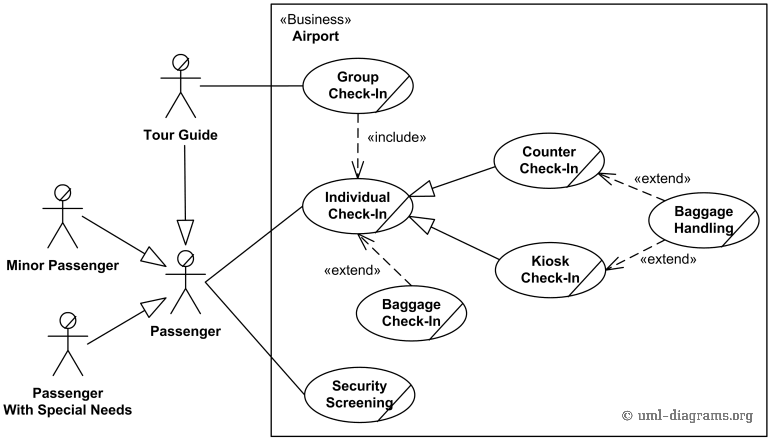
\includegraphics[width=0.7\textwidth]{airportUseCase.png}
    \attribution{\url{http://www.uml-diagrams.org}}
\end{center}

Тут показано ещё и наследование --- как между акторами, так и между случаями использования. Наследование, как обычно, является способом классификации сущностей --- например, пассажир бывает малолетним, инвалидом или экскурсоводом. И если пассажирам вообще доступна индивидуальная регистрация и досмотр (вряд ли досмотр можно назвать целью пассажиров, но всё же), то экскурсоводу помимо всего этого доступна ещё и групповая регистрация. То же касается случаев использования --- регистрация бывает у стойки, а бывает через терминал. В любом случае, если у пассажира есть багаж, его надо сдать, и на то есть свой случай использования, являющийся расширением первых двух. А групповая регистрация состоит из набора индивидуальных регистраций, поэтому отношение <<include>>.

\subsubsection{Сценарии использования}

Каждый случай использования раскрывается в один или несколько сценариев использования. Иногда используются формальные описания сценариев использования, рассмотрим их, чтобы понимать, что вообще там надо писать.

Типичная структура сценария использования такова.

\begin{itemize}
    \item Заголовок --- цель основного актора, собственно, случай использования.
    \item Заинтересованные лица, акторы, основной актор --- сюда выписываются все роли, участвующие в сценарии, среди них выделяется одна --- которая инициирует исполнение сценария.
    \item Предусловия --- какие логические условия должны быть истинны, чтобы сценарий в принципе мог быть исполнен.
    \item Триггеры (активаторы) --- что должно произойти, чтобы сценарий начал выполняться, при условии, что все предусловия выполнены.
    \item Основной порядок событий --- что происходит, если всё идёт по плану. Сюда пишется наиболее типичная последовательность действий.
    \item Альтернативные пути и расширения --- сюда пишется, что делать в нетипичной ситуации, тут же описываются точки расширения и реакция на ошибки.
    \item Постусловия --- какие логические условия должны быть истинны после исполнения сценария.
\end{itemize}

Вот пример карточки сценария использования, сделанной по такой структуре (из книги  R.M. Roth et al., System Analysis and Design):

\begin{center}
    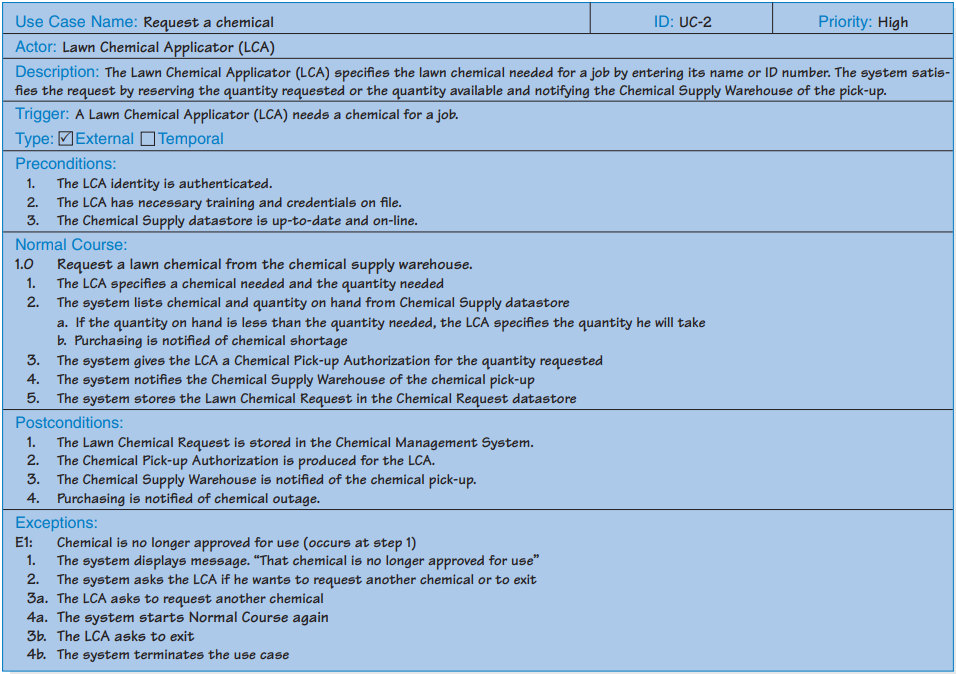
\includegraphics[width=0.95\textwidth]{useCaseExample.png}
    \attribution{R.M. Roth et al., System Analysis and Design}
\end{center}

\subsection{Контекстная диаграмма IDEF0}

Диаграммы случаев использования хороши тем, что они очень просты и ни к чему не обязывают (из всего UML можно использовать только их, и они легко вписываются в любую методологию), так что применяются даже в Agile-командах иногда. Но есть ещё более простая нотация (и гораздо более древняя): контекстные диаграммы языка IDEF0.

Вообще языки семейства IDEF (Integration DEFinition, в оригинале --- ICAM DEFinition) разрабатывались аж в 1970-х годах по заказу минобороны США, когда у тех возникла потребность в разработке сложного mission-critical программного обеспечения и подхода <<фигачить код>> стало не хватать. Семейство на данный момент включает в себя 14 языков (как UML), но широкую известность получили только IDEF0 и IDEF1x, так что упоминаются в этом курсе только они.

Нотация IDEF0 (так же известная как SADT, Structured Analysis and Design Technique, хотя это не совсем верно, SADT появился раньше) используется для структурной декомпозиции системы (или бизнес-процесса, в который система встраивается). Процесс представляется в виде набора шагов, соединённых входами и выходами друг с другом. Диаграммы выглядят примерно вот так:

\begin{center}
    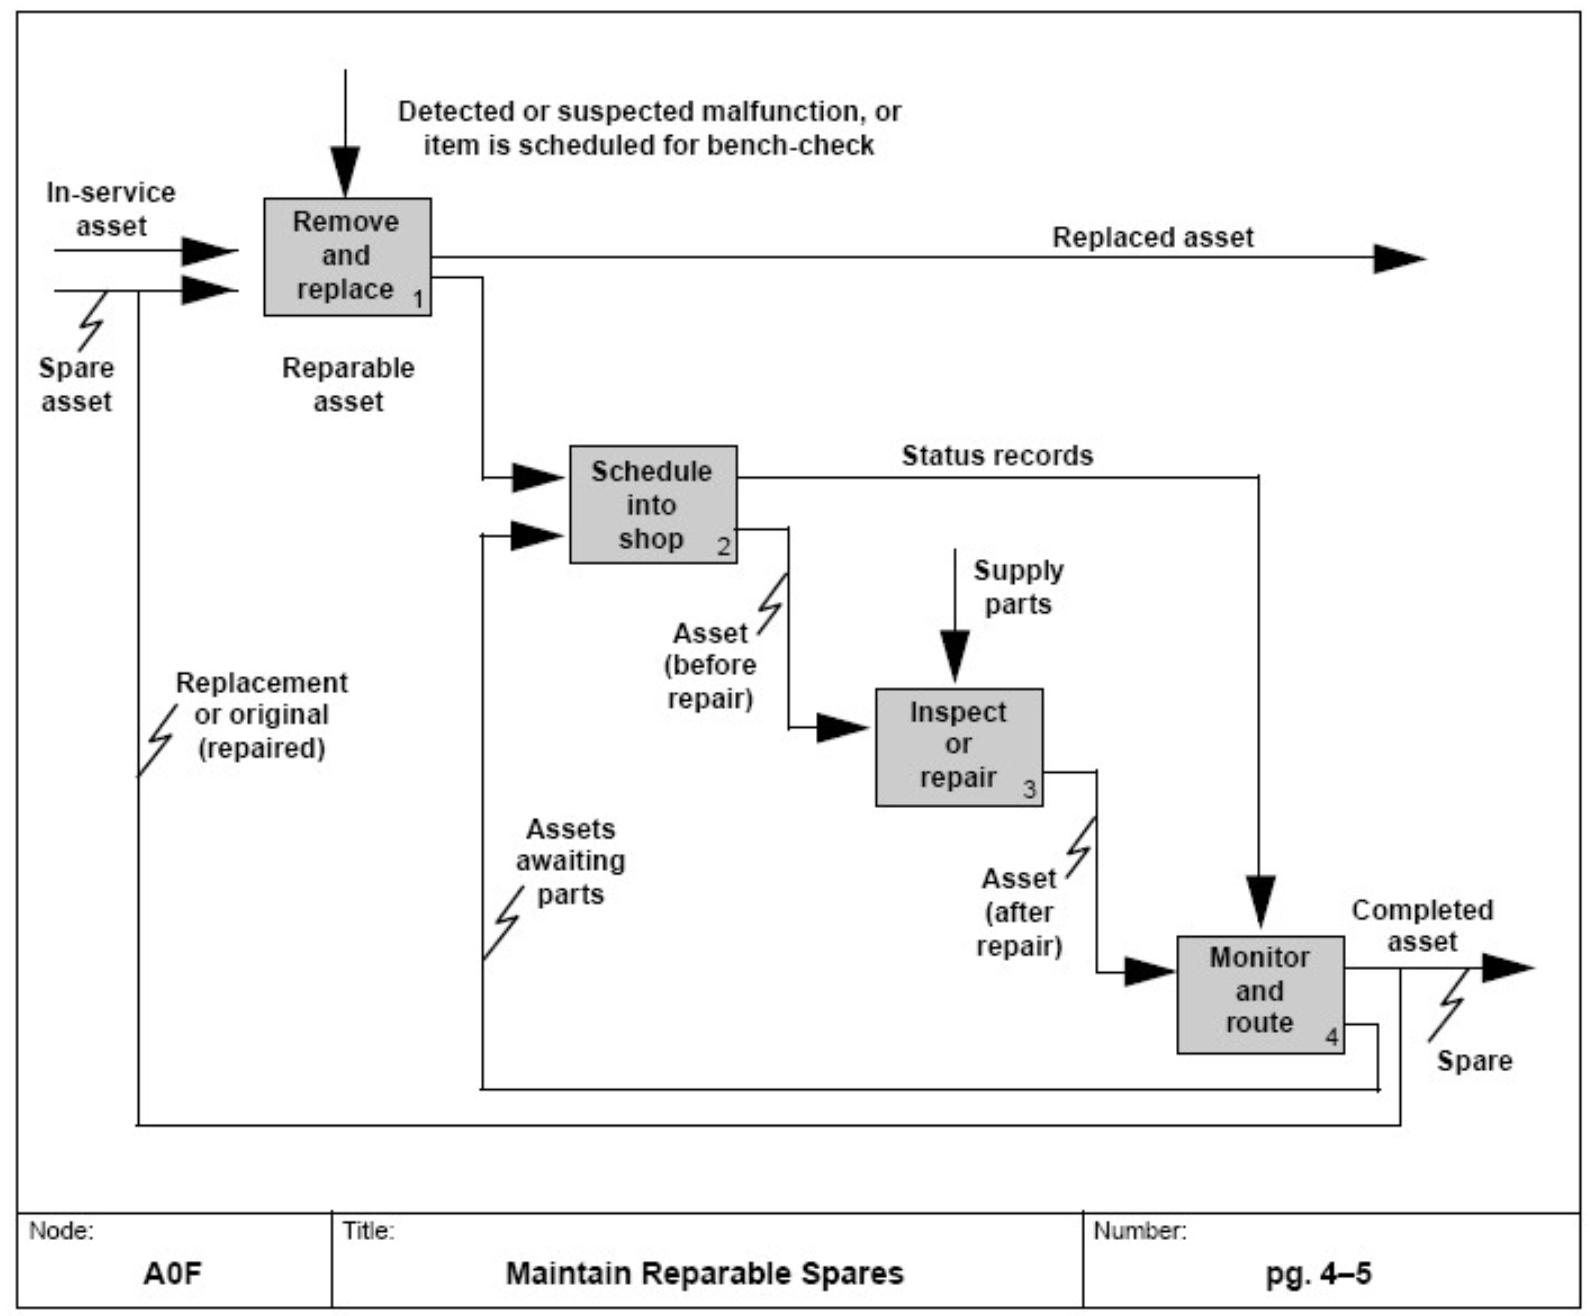
\includegraphics[width=0.7\textwidth]{idef0.png}
    \attribution{https://en.wikipedia.org/wiki/IDEF0}
\end{center}

Выходов у каждого блока всего один тип, хотя и может быть много, а вот входов три разных типа:

\begin{center}
    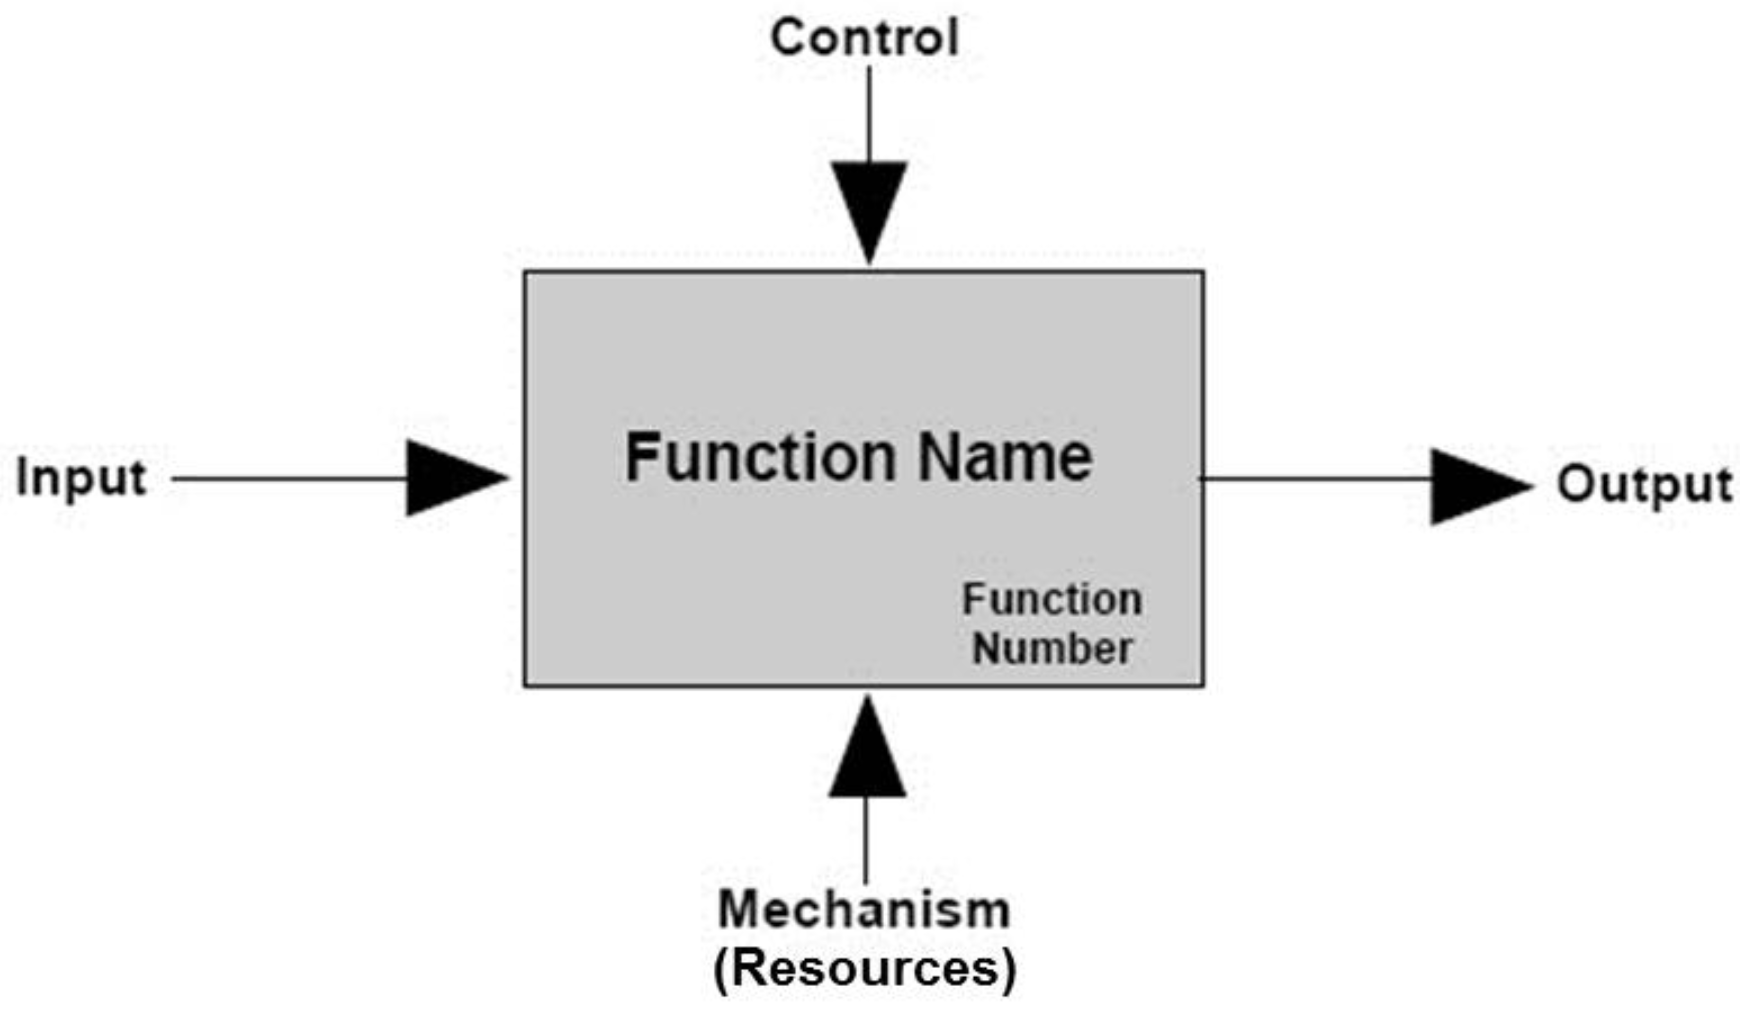
\includegraphics[width=0.4\textwidth]{idef0block.png}
    \attribution{https://en.wikipedia.org/wiki/IDEF0}
\end{center}

Слева --- входы блока, материалы, которые он перерабатывает в то, что получается на выходе. Сверху --- управление, то есть то, что определяет, как блок работает (например, настройки или должностные инструкции). Снизу --- механизмы, то есть то, что позволяет блоку работать (например, база данных или станки на конвейере). Опять-таки, входов каждого типа может быть много.

Каждый блок может быть далее раскрыт своей IDEF0-диаграммой, при этом все входы на исходной диаграмме должны быть входами и на диаграмме, раскрывающей блок, аналогично с выходами --- каждую связь должно быть можно отследить.

В корне иерархии диаграмм лежит та самая контекстная диаграмма IDEF0, которая нам и интересна в плане работы с требованиями. На ней рисуется всего один блок, означающий вообще всю систему. Входящими стрелками показываются входы, механизмы и управление для системы, приходящие извне (именно извне, всякие внутренние дела системы на этой диаграмме не рисуются), выходами --- то, что полезного получается в результате работы системы. Небольшой пример (не из мира ПО, правда, но IDEF0 вообще чаще используются для моделирования бизнес-процессов и производственных процессов, чем для моделирования ПО, UML же есть --- однако именно модели бизнес-процессов и нужны для того, чтобы грамотно описать требования):

\begin{center}
    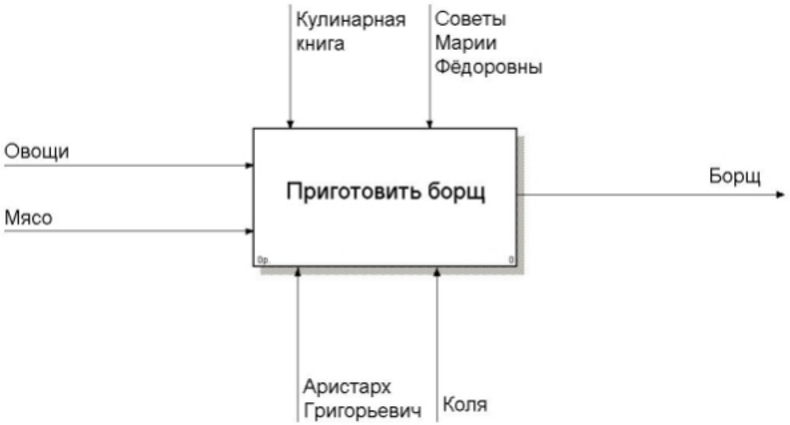
\includegraphics[width=0.5\textwidth]{idef0Example.png}
    \attribution{https://en.wikipedia.org/wiki/IDEF0}
\end{center}

Такая диаграмма кажется настолько простой, что полезность её сомнительна, но именно в этом её преимущества --- она позволяет чётко определить границу системы, её входы и выходы, так, чтобы это помещалось на одном экране.

\subsection{Диаграмма характеристик}

Контекст, в котором система работает --- это хорошо, но недостаточно, чтобы начать её реализовывать, нужны конкретные требования. Требования обычно иерархичны, поэтому и представлять их удобнее всего в виде дерева. Чаще всего это делают текстом, в виде списков, но есть и визуальная нотация: диаграмма характеристик (feature diagram). Выглядит она как-то так:

\begin{center}
    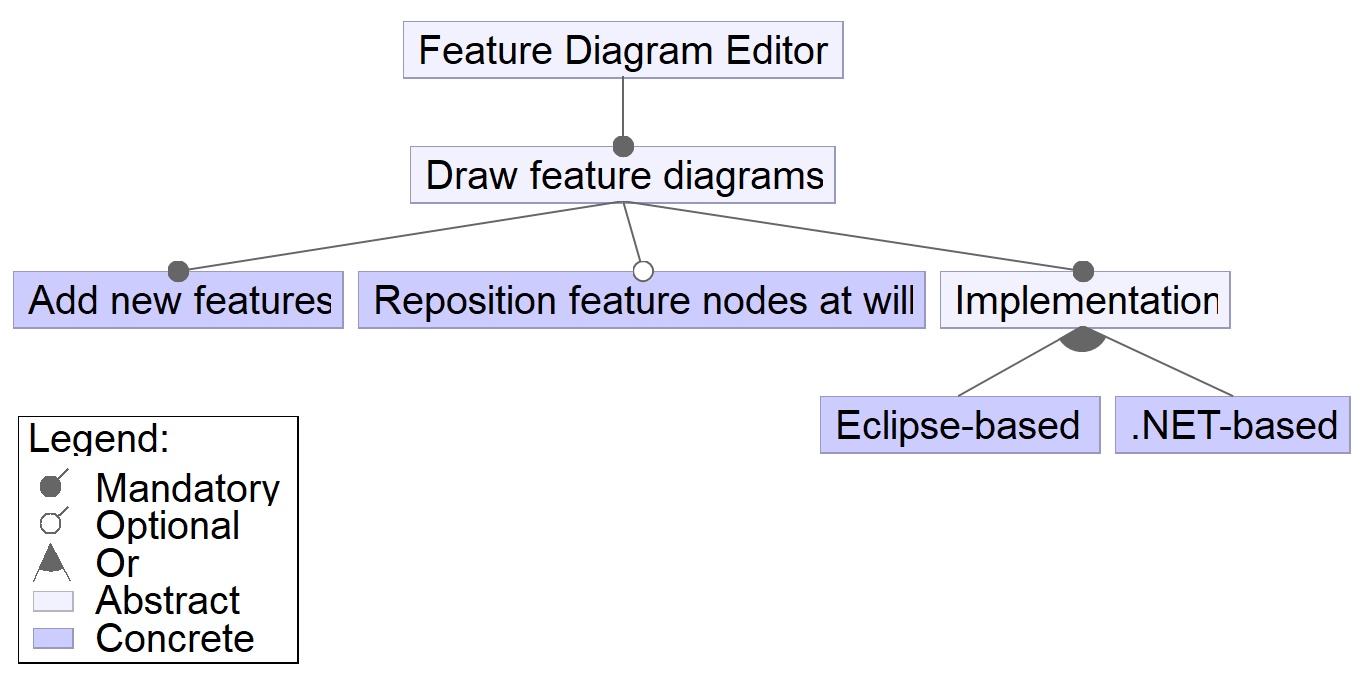
\includegraphics[width=0.7\textwidth]{featureDiagram.png}
\end{center}

Нотация очень простая --- характеристики бывают абстрактными (то есть теми, которые надо ещё декомпозировать перед тем как реализовать) и конкретными (пригодными к реализации), отношения между характеристиками бывают <<или>> (включающее и исключающее), обязательность и необязательность (то есть, без необязательной характеристики продукт вполне может существовать).

Для <<повседневного>> анализа требований диаграммы характеристик не очень удобны (отчасти потому, что их почти никто из CASE-систем не поддерживает, отчасти потому, что они получаются очень большими). Однако они активно используются в разработке линеек программных продуктов (например, если у вас есть Professional и Ultimate-версии, то можно отметить на общей диаграмме характеристик, какие характеристики куда попадают). Особенно хорошо это работает, если можно наладить автоматическую генерацию конфигурации продукта (или даже кода) по диаграммам.

Хороший пример такого подхода описан в статье D. Brugali et al., ``Variability Modeling of Service Robots Experiences and Challenges'' (2019) (точнее, у них про это целый проект BRICS, публикаций по нему много, эта даже не самая показательная, но относительно свежая). Товарищи занимаются конфигурированием ПО для сервисных роботов, что особенно сложно, потому что роботы имеют разную аппаратную конфигурацию, работают в разном окружении и предназначены для разных задач. Поэтому и программные платформы, и конкретное ПО приходится выбирать из массы вариантов и адаптировать под конкретного робота, задачи и даже аппаратная конфигурация которого может меняться по ходу дела.

Общая идея такая: описать все возможные характеристики аппаратной платформы, характеристики доступного ПО и получить диаграммы характеристик в духе:

\begin{center}
    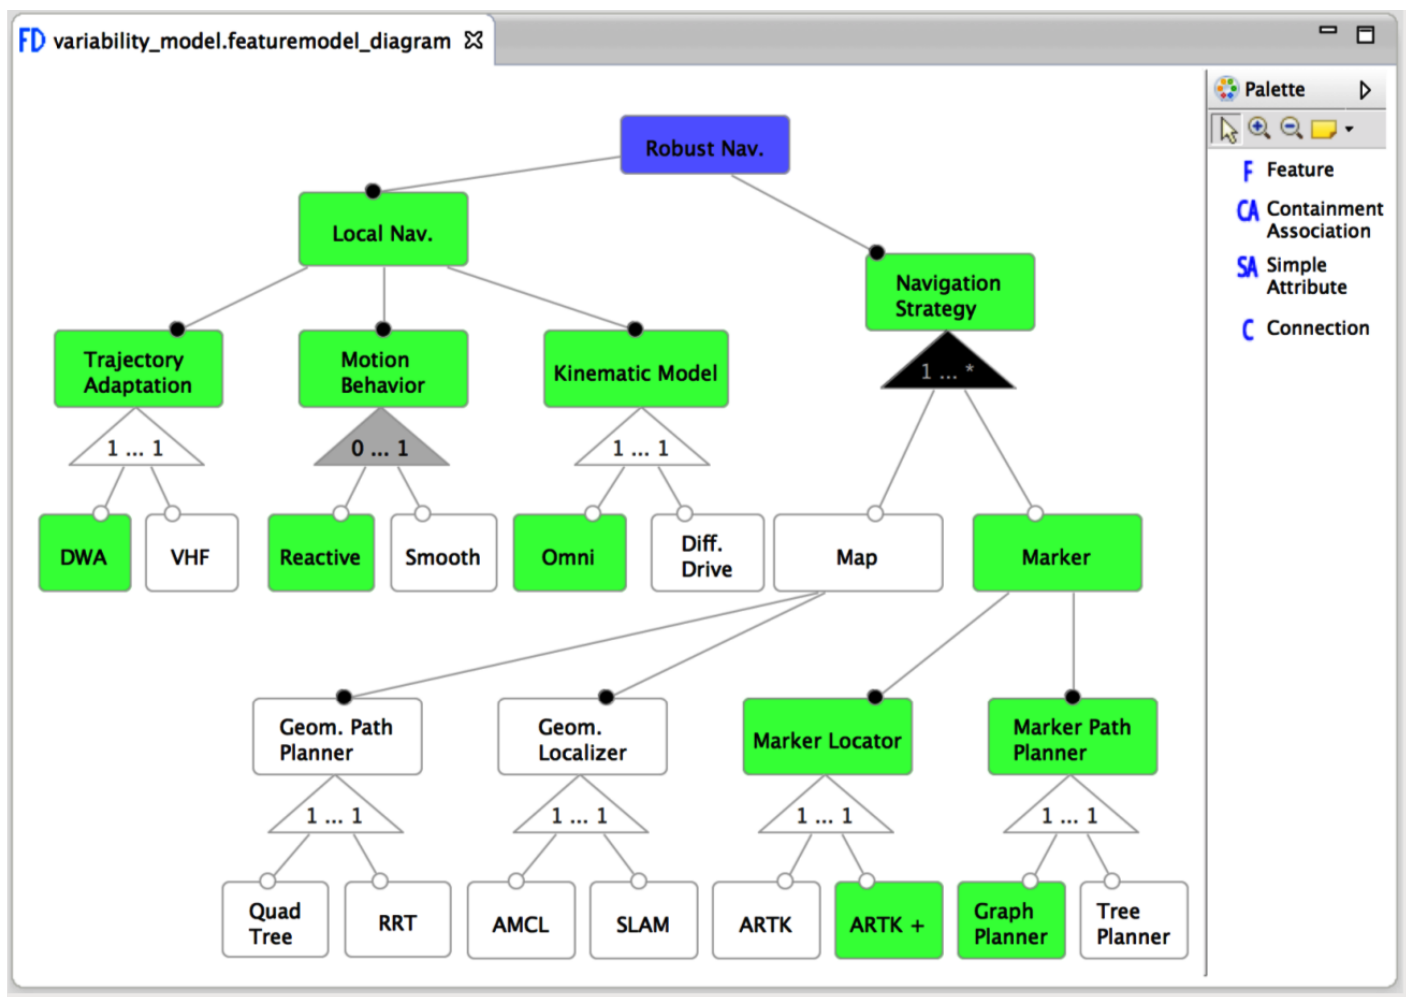
\includegraphics[width=0.9\textwidth]{featureDiagramExample.png}
    \attribution{D. Brugali et al.}
\end{center}

Дальше под конкретную задачу можно просто выбирать нужные характеристики, а система сама сгенерирует код, который развернёт на роботе нужный софт и правильно его сконфигурирует. На самом деле, там не всё так просто, есть ещё отображения между характеристиками аппаратной платформы и характеристиками ПО, зависимости между характеристиками (например, если на роботе нет камеры, то распознавать маркеры на стенах не выйдет), есть типовая архитектура, которая, собственно, позволяет конфигурировать систему, но это уже детали реализации и не относится к теме лекции.

\subsection{Feature tree}

Диаграммы характеристик довольно громоздки и их сложно рисовать, поэтому во время первоначального анализа требований (например, brainstorm-а по поводу нового проекта) можно использовать похожую, но более простую нотацию: дерево характеристик (feature tree, или их ещё называют fishbone diagram из-за внешней схожести со скелетом рыбы). Выглядят они так:

\begin{center}
    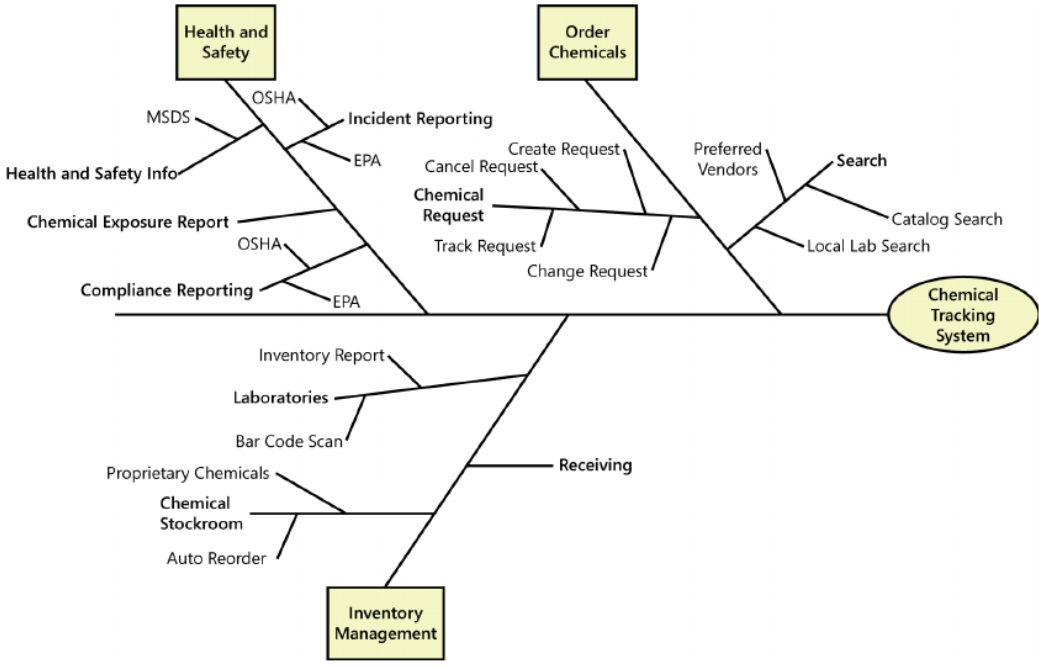
\includegraphics[width=0.7\textwidth]{featureTree.png}
\end{center}

<<Голова рыбы>> --- это система в целом, от неё отходит <<хребет>>, от которого отходят основные фичи. Они дальше детализируются более мелкими фичами, рисуемыми как ответвления от основных. На такой диаграмме никаких взаимосвязей не показать, но как инструмент первоначального анализа она может быть очень полезна. А потом уже можно нарисовать случаи использования, диаграмму характеристик и т.д.

\subsection{Диаграмма требований SysML}

Есть более формальная нотация дерева требований, в языке SysML. SysML изначально создавался как профиль (т.е. стандартное расширение) языка UML для моделирования больших систем, включавших в себя как программные, так и аппаратные компоненты, а так же людей и другие системы. Потом этот язык стал отдельным языком, туда добавили несколько новых видов диаграмм (которые будут упомянуты дальше в курсе), в частности, диаграмма требований. Выглядит она так:

\begin{center}
    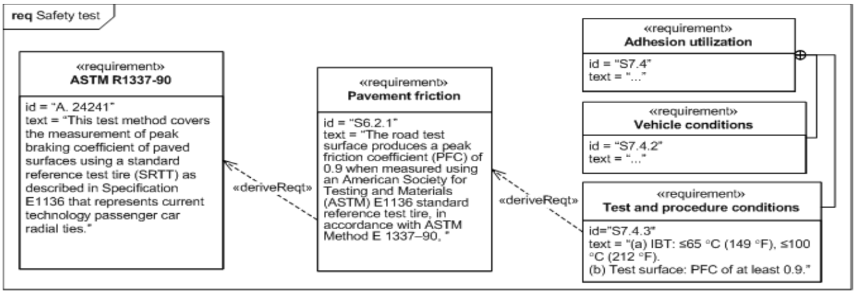
\includegraphics[width=0.8\textwidth]{sysMlRequirementDiagram.png}
    \attribution{OMG SysML 1.4 Specification}
\end{center}

Требования рисуются похоже на классы, со стереотипом \verb|<<requirement>>|, именем и идентификатором требования, и, главное, текстовым описанием. Требования могут находиться в разных отношениях (например, \verb|<<deriveReqt>>|, означающее, что одно требование является уточнением другого, или \verb|satisfy|, означающее, что какой-то элемент системы, например, класс, удовлетворяет или реализует то или иное требование).

Вот более содержательный пример:

\begin{center}
    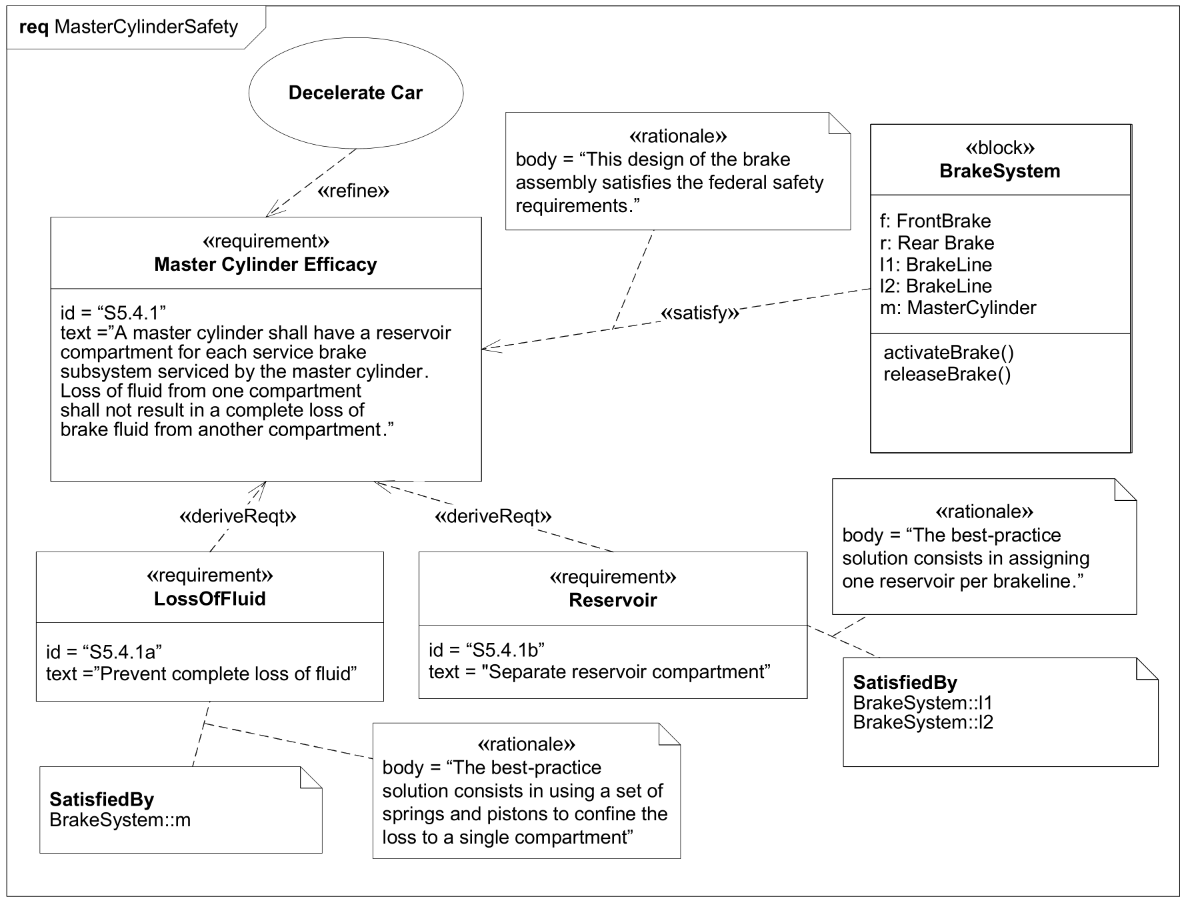
\includegraphics[width=0.7\textwidth]{sysMlRequirementsExample.png}
    \attribution{OMG SysML 1.4 Specification}
\end{center}

Как видим, на одной диаграмме могут рисоваться совершенно разные элементы. Случай использования <<Decelerate Car>> уточняется требованием <<Master Cylinder Efficacy>>, которое реализуется подсистемой <<BrakeSystem>> (классы и целые подсистемы в SysML называются блоками). При этом <<Master Cylinder Efficacy>> уточняется наличием требования на невозможность полной потери тормозной жидкости и наличием раздельных резервуаров тормозной жидкости для каждой из линий тормозной системы. Каждое требование поясняется комментарием \verb|<<rationale>>|, где написано, почему было принято такое решение.

Требования могут быть также уточнены сценарием тестирования (в SysML даже есть стандартные отношения \verb|<<verifies>>|/\verb|<<verifiedBy>>|). Сценарий тестирования может быть представлен в виде диаграммы активностей. Например, требования на работу тормозных колодок:

\begin{center}
    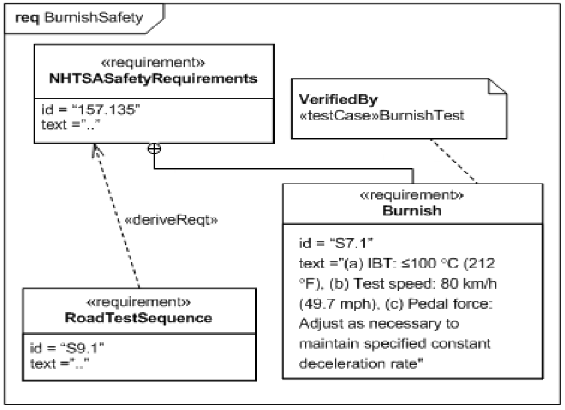
\includegraphics[width=0.5\textwidth]{sysMlRequirementsTest.png}
    \attribution{OMG SysML 1.4 Specification}
\end{center}

могут быть проверены следующим сценарием тестирования:

\begin{center}
    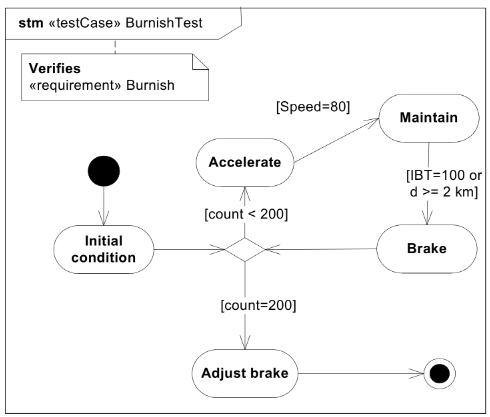
\includegraphics[width=0.5\textwidth]{sysMlRequirementsTestActivity.png}
    \attribution{OMG SysML 1.4 Specification}
\end{center}

\section{Моделирование бизнес-процессов}

\subsection{Диаграмма активностей UML}

Важной задачей на этапе анализа, помимо сбора требований, является ещё и анализ бизнес-процессов, которые (или часть которых) мы хотим автоматизировать. Для этого применяются несколько нотаций --- во-первых, диаграммы активностей UML, во-вторых, отдельный язык BPMN (Business Process Model and Notation), который, как и UML, состоит из нескольких видов диаграмм и специально предназначен для моделирования бизнес-процессов.

Но сначала про диаграммы активностей из UML, как более легковесный инструмент. Внешне они очень напоминают блок-схемы, но используются прежде всего не для моделирования алгоритмов (хотя и для этого тоже, иногда), а для моделирования поведения бизнес-процесса в целом. Кстати, термином <<бизнес-процесс>> в IT принято называть любой процесс работы в организации, может быть, и не связанный с бизнесом. Зачем вообще моделировать процессы --- во-первых, для того, чтобы понять, как в существующий процесс вписывается разрабатываемая система, во-вторых, это хороший способ визуализации сценария использования системы, с точки зрения пользователя.

Кстати, это одна из двух диаграмм UML, для которой описана семантика её исполнения, на основе сетей Петри. Вторая диаграмма --- это диаграмма конечных автоматов, про которую несколько попозже. Выглядит диаграмма активностей (также иногда встречается вариант перевода <<диаграмма деятельностей>>) так:

\begin{center}
    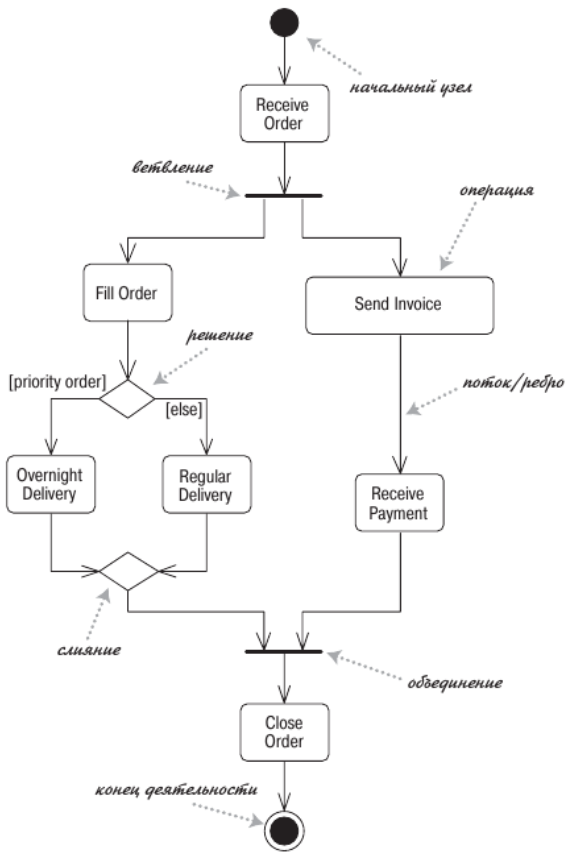
\includegraphics[width=0.5\textwidth]{activityDiagram.png}
    \attribution{М. Фаулер, UML. Основы}
\end{center}

<<Ветвление>>/<<объединение>> работает как fork/join для параллельных потоков --- <<ветвление>> разделяет исполнение на два или больше параллельных потоков, <<объединение>> ждёт, пока все входящие в него потоки закончат исполнение, и только после этого отдаёт управление дальше. Ничто не мешает потоки не объединять, тогда исполнение заканчивается, как только хотя бы один поток дойдёт до блока <<конец деятельности>>. По синтаксису каждый блок <<решение>> может иметь несколько веток (в этом смысле он похож на оператор switch/case в текстовых языках), но все ветки должны сходиться на блоке <<слияние>>. Причём, в отличие от блок-схем, условие пишется не в ромбике, а над каждой исходящей стрелкой, и условия должны быть взаимоисключающими.

Ещё на диаграмме активностей можно показать разделение работ по отделам организации или частям системы. Это важно в анализе бизнес-процессов, поскольку визуализирует разделение ответственности между частями организации. Рисуются разделы так:

\begin{center}
    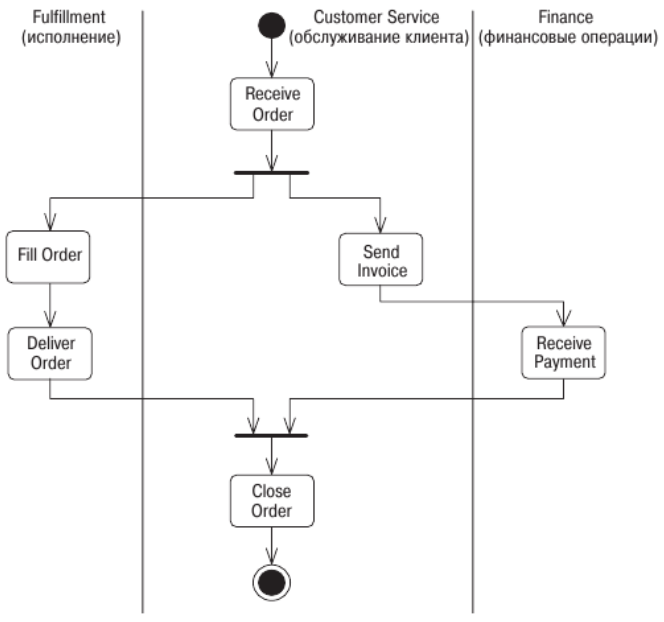
\includegraphics[width=0.5\textwidth]{activitySwimlanes.png}
    \attribution{М. Фаулер, UML. Основы}
\end{center}

А ещё, в отличие от блок-схем, есть возможность показать асинхронное взаимодействие с помощью сигналов. Рисуются они вот так:

\begin{center}
    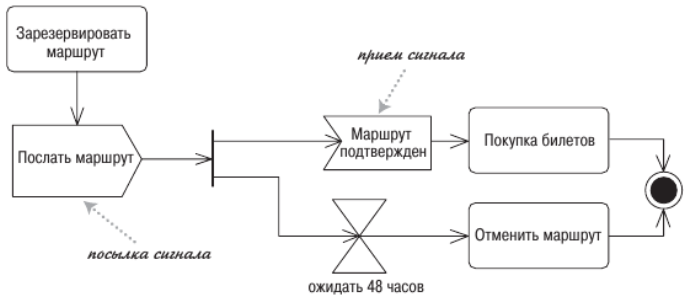
\includegraphics[width=0.6\textwidth]{activitySignals.png}
    \attribution{М. Фаулер, UML. Основы}
\end{center}

Сигналом чаще всего является отправка документа, но может быть и сетевой запрос, и электронное письмо, и что-то ещё, что отправляется за границы моделируемого бизнес-процесса. Блок <<посылка сигнала>> тут же возвращает управление и процесс продолжается вне зависимости от того, принял кто-то сигнал или нет. Блок <<приём сигнала>> ждёт указанный сигнал и продолжает процесс только когда сигнал поступит. Ещё есть блок <<таймер>>, который можно понимать как отложенный сигнал самим себе --- процесс ждёт указанное время, затем продолжается. На диаграмме выше показан типичный запрос с таймаутом.

\subsection{Business Process Model and Notation}

Для более продвинутого анализа бизнес-процессов используется отдельный язык BPMN (Business Process Model and Notation), который не входит в UML, хотя и является его близким родственником. Диаграммы активностей хороши, если у вас один-два бизнес-процесса с тремя-четырьмя участниками, однако в реальной жизни нередки ситуации, когда у организации более сотни субподрядчиков, и взаимодействие с каждым --- отдельный бизнес-процесс, а работа организации --- это тоже бизнес-процесс, включающий в себя эти бизнес-процессы. Если вдруг не повезло автоматизировать бизнес-процессы такого масштаба, то без BPMN не обойтись. Правда, в этом случае не стоит доверять анализ бизнес-процессов архитектору, лучше нанять отдельного бизнес-аналитика. Поэтому BPMN несколько реже встречается в программистской практике, чем диаграммы активностей UML, и поэтому в этом курсе про BPMN будет существенно меньше, чем могло бы быть, но поскольку архитектору надо как-то общаться с аналитиками и вообще знать, что такое бывает, про BPMN всё-таки будет.

Стандарт BPMN 1.0 был принят в 2004 году, как раз примерно в те времена, что и UML 2.0, тем же консорциумом Object Management Group, который управляет UML. BPMN также определён с помощью метамодели и стандарты очень похожи по принципам определения языка, но BPMN, тем не менее, отдельный язык (точнее, как и UML, набор языков).

BPMN можно воспринимать как сильно продвинутые диаграммы активностей. Он позволяет, в частности, визуализировать взаимодействие нескольких процессов (в отличие от диаграмм активностей, где посылка и приём сигналов просто не связанные между собой блоки, в BPMN рисуются нормальные стрелочки), имеет гораздо больший набор блоков-ветвлений (в том числе и с параллельными потоками), блоков ожидания разных событий, качественную поддержку исключений. Так же, как и диаграммы активностей, BPMN имеет исполнимую семантику, но, в отличие от диаграмм активностей, эта семантика может быть использована для реального исполнения бизнес-процесса в информационной системе --- благодаря стандартизованным правилам преобразования диаграмм на BPMN в XML-документы на BPEL (Business Process Execution Language), настоящем исполнимом языке описания бизнес-процессов, который поддерживают многие движки-исполнители\footnote{см. \url{https://en.wikipedia.org/wiki/List_of_BPEL_engines}}.

\subsubsection{Диаграмма процессов}

Вот так выглядит самая, пожалуй, известная диаграмма BPMN (которую часто путают с BPMN вообще, например, в википедии) --- диаграмма процессов (process diagram):

\begin{center}
    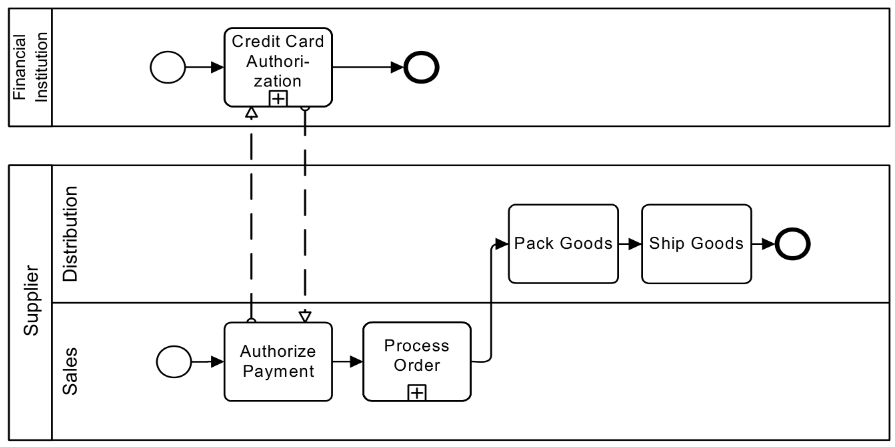
\includegraphics[width=0.9\textwidth]{bpmnExample.png}
    \attribution{OMG BPMN 2.0 Specification}
\end{center}

Тут изображены два бизнес-процесса двух независимых организаций, общающихся посылкой и приёмом сообщений. Бизнес-процесс одной из огранизаций поделен на два раздела, но тем не менее, это один бизнес-процесс, на что указывает единый поток управления. Плюсик внутри активности означает, что активность раскрывается в другой, более детализированный бизнес-процесс. Пользоваться такими диаграммами можно как диаграммами активностей UML, а подробнее прочитать про их синтаксис можно, как ни странно, в русской википедии (\url{https://ru.wikipedia.org/wiki/BPMN}), если не хотите ознакомиться с почти шестисотстраничным стандартом\footnote{\url{https://www.omg.org/spec/BPMN/2.0/}}. Вот табличка с видами событий оттуда:

\begin{center}
    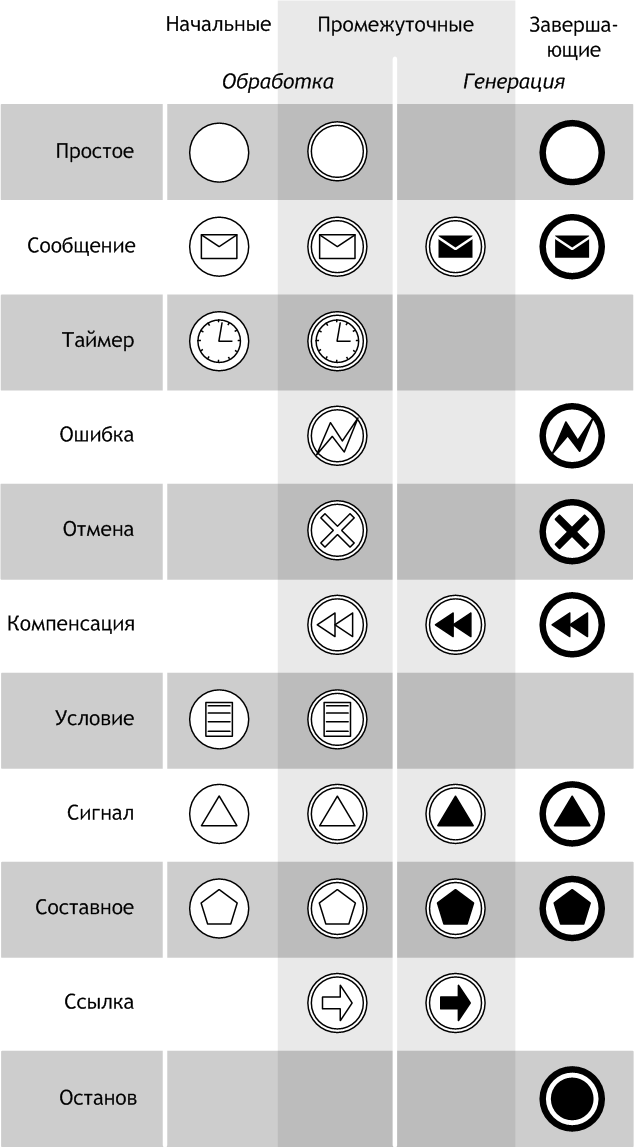
\includegraphics[width=0.4\textwidth]{bpmnEvents.png}
    \attribution{\url{https://ru.wikipedia.org/wiki/BPMN}}
\end{center}

Пояснять тут её нет смысла, потому что в википедии всё подробно описано, но представление о том, что в BPMN бывает и почему BPMN лучше для анализа сложных процессов, чем диаграмма активностей UML, это даёт. А вот несколько менее эпичная таблица с типами логических операторов (опять же, из википедии, и, опять же, без пояснений):

\begin{center}
    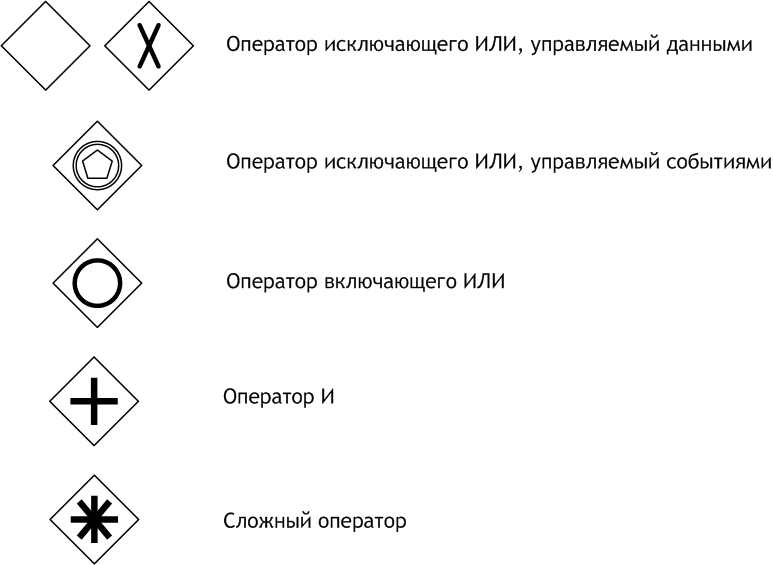
\includegraphics[width=0.5\textwidth]{bpmnGateways.png}
    \attribution{\url{https://ru.wikipedia.org/wiki/BPMN}}
\end{center}

\subsubsection{Диаграмма хореографии}

Второй вид диаграмм BPMN --- диаграмма хореографии (choreography diagram) --- описывает исключительно взаимодействие между бизнес-процессами. На ней не рисуется кто что должен делать, на ней рисуется, кто когда с кем должен общаться. Выглядит это так:

\begin{center}
    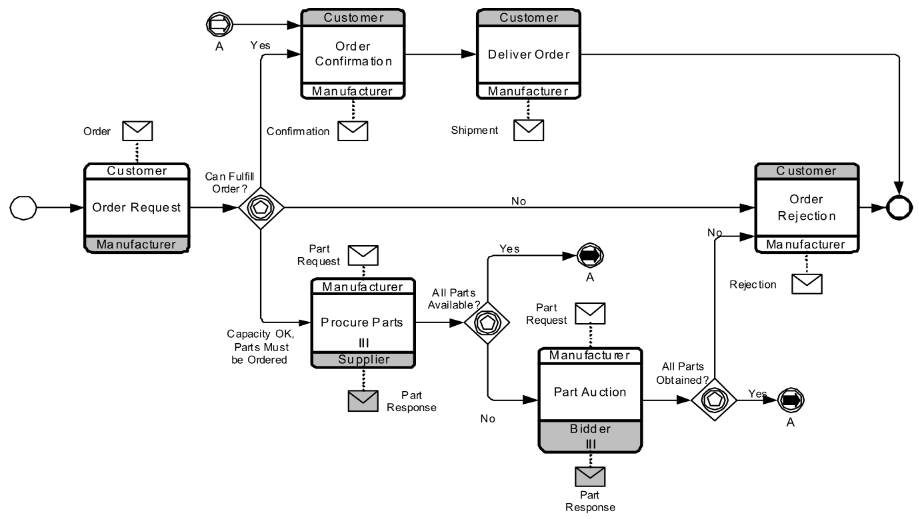
\includegraphics[width=0.9\textwidth]{bpmnChoreography.png}
    \attribution{OMG BPMN 2.0 Specification}
\end{center}

Прямоугольники со скруглёнными углами --- это точки общения между процессами, белым цветом выделен инициатор взаимодействия, серым --- тот, кто должен ему ответить, конвертиком --- сообщение или документ. Как видим, ветвления и события тут рисуются, а активности --- нет. Такая диаграмма нужна, если попытка изобразить процессы в дорожках на диаграмме процессов привела бы к хаосу из стрелочек.

\subsubsection{Диаграмма диалогов}

И последняя диаграмма BPMN --- диаграмма диалогов (conversation diagram), она показывает схему общения бизнес-процессов, не в смысле когда кто с кем общается, как диаграмма хореографии, а в смысле кто с кем в принципе может общаться. Выглядит диаграмма вот так:

\begin{center}
    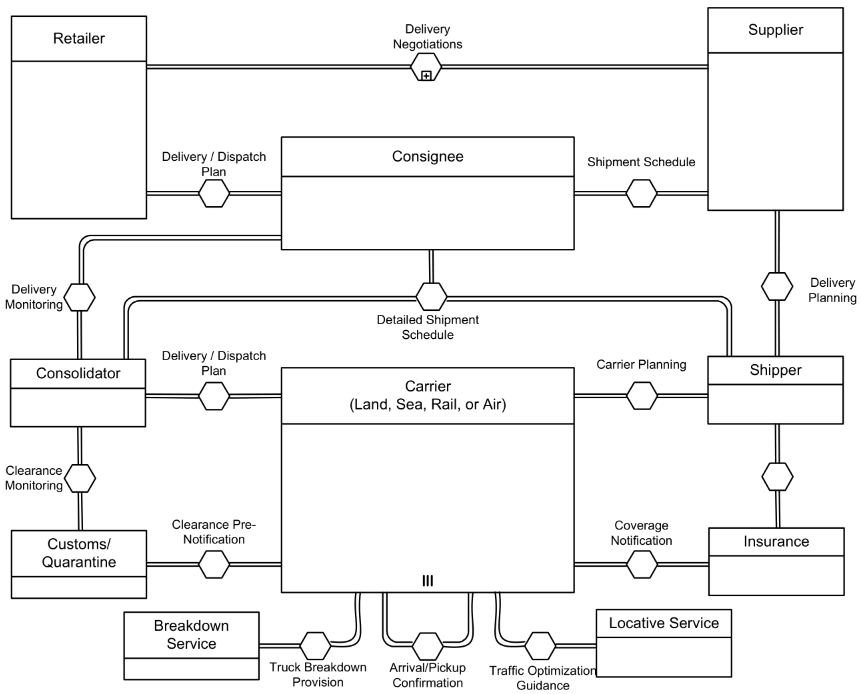
\includegraphics[width=0.9\textwidth]{bpmnConversation.png}
    \attribution{OMG BPMN 2.0 Specification}
\end{center}

Прямоугольниками показаны участники взаимодействия, двойными линиями с шестиугольниками --- общение между участниками. Плюсик внутри шестиугольника показывает, что взаимодействий между участниками много и они могут быть уточнены диаграммами хореографий или диаграммами процессов без деталей (это когда просто рисуются дорожки и сообщения, без внутреннего содержимого, так тоже можно). Три вертикальные черты внутри участника взаимодействия означают, что участников на самом деле может быть много.

На этом закончим обзор BPMN (очень-очень краткий, там ещё куча разных тонкостей, про которые надо знать, чтобы стать нормальным аналитиком, но у нас тут курс по архитектуре). Можно дополнительно ознакомиться с примерами BPMN-диаграмм из небольшого, неформального, но очень полезного документа от OMG: \url{https://www.omg.org/cgi-bin/doc?dtc/10-06-02}

\section{Диаграмма развёртывания UML}

Диаграмма развёртывания UML (deployment diagram) используется для того, чтобы показать размещение логических элементов системы (компонентов, исполнимых файлов) на физических или виртуальных устройствах. Пример такой диаграммы:

\begin{center}
    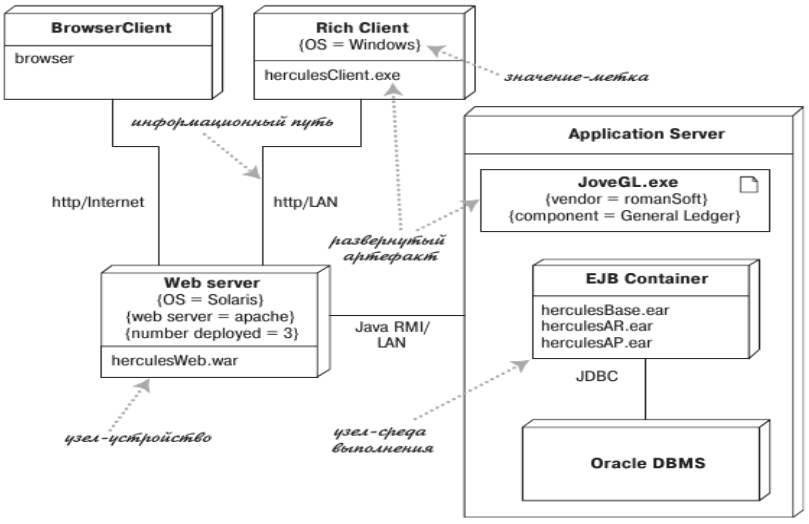
\includegraphics[width=0.7\textwidth]{deploymentDiagram.png}
    \attribution{М. Фаулер, UML. Основы}
\end{center}

Параллелепипедами на диаграмме рисуются устройства или похожие на устройства части системы (реальные компьютеры или группы компьютеров, базы данных, среды выполнения и т.д.). В них рисуются развёрнутые там артефакты (бинарники, компоненты и т.д.). Связи здесь возможны только между узлами (устройствами) и показывают они физические (или низкоуровневые логические) каналы связи между узлами, с указанием протокола взаимодействия. И узлы, и артефакты могут иметь дополнительные свойства, пишушиеся в фигурных скобках. Артефакты можно рисовать как подробно (прямоугольником), так и кратко (просто надписью с именем артефакта).

Казалось бы, развёртывание происходит ближе к концу разработки, так что не имеет отношения к анализу. Однако оказывается, что часто физические устройства известны заранее (например, заказчик уже купил два сервера и готов купить ещё пяток терминалов), и наличествующие физические устройства во многом определяют архитектуру системы. Тогда диаграмма развёртывания очень полезна как инструмент именно анализа --- она позволяет отобразить уже существующую инфраструктуру и понять, как мы намерены её использовать.

Ещё одно полезное применение диаграммы развёртывания --- обратное проектирование, когда система у заказчика уже есть, но никто не знает, как она устроена, а вам надо для неё чего-то написать. Как правило, даже если документация по коду совсем не сохранилась, у админов есть документация по сопровождению, или они просто знают, какую машину надо перезапустить, если повис такой-то сервис. Если отобразить эти знания на диаграмме развёртывания, получим первое приближение высокоуровневой архитектуры системы.

\section{Моделирование данных}

\subsection{Диаграммы <<Сущность-связь>>}

Следующая важная часть анализа предметной области --- это анализ данных, с которыми предстоит работать нашей программе. Точнее даже поначалу анализ сущностей, наличествующих в предметной области, их взаимосвязей и свойств. Для этого тоже есть несколько визуальных языков, но, поскольку построению схем БД обычно хорошо учат на курсе по базам данных, тут только затронем этот вопрос, и то только его визуальную составляющую. В данном случае ситуация несколько обратна BPMN --- моделирование сущностей и связей предметной области и создание концептуальной схемы базы данных --- это одна из основных деятельностей архитектора, но раз она хорошо покрыта другими курсами, мы тоже только слегка её затронем.

Итак, для описания концептуальной модели предметной области чаще всего используются диаграммы <<сущность-связь>> (хотя могут и диаграммы классов UML). Для построения схемы реляционной базы данных используются практически исключительно диаграммы <<сущность-связь>>, поскольку они семантически очень хорошо ложатся в реляционную модель данных. Хитрость в том, что у диаграмм <<сущность-связь>> есть несколько нотаций.

Первая нотация была предложена Питером Ченом ещё в 1976 году и выглядит так:

\begin{center}
    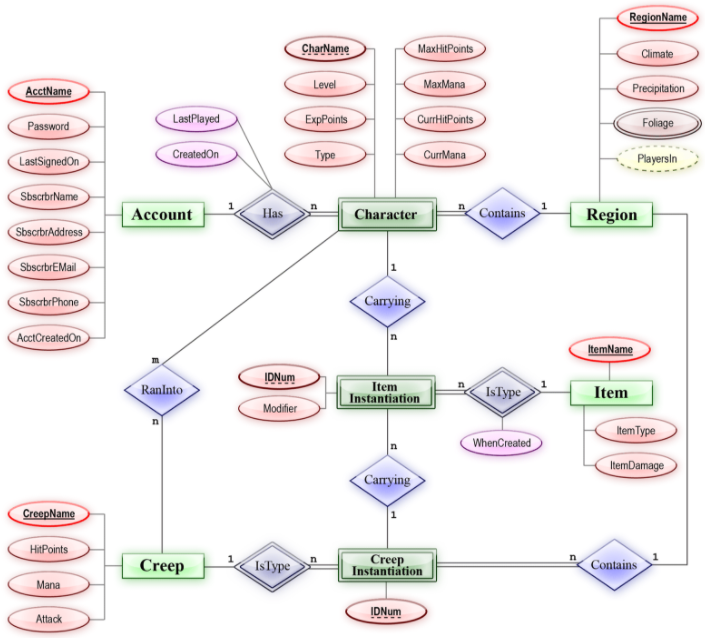
\includegraphics[width=\textwidth]{erChenNotation.png}
    \attribution{https://ru.wikipedia.org}
\end{center}

Прямоугольники означают сущности, овалы --- их свойства, ромбы --- связи между сущностями (которые сами могут иметь какие-то свойства). Связи могут иметь кратность (один к одному, один ко многим, даже многие ко многим), какой-то атрибут может быть назначен первичным ключом. Никогда не видел, чтобы эта нотация использовалась на практике.

Реально используются сейчас разные варианты нотации <<вороньей лапки>>:

\begin{center}
    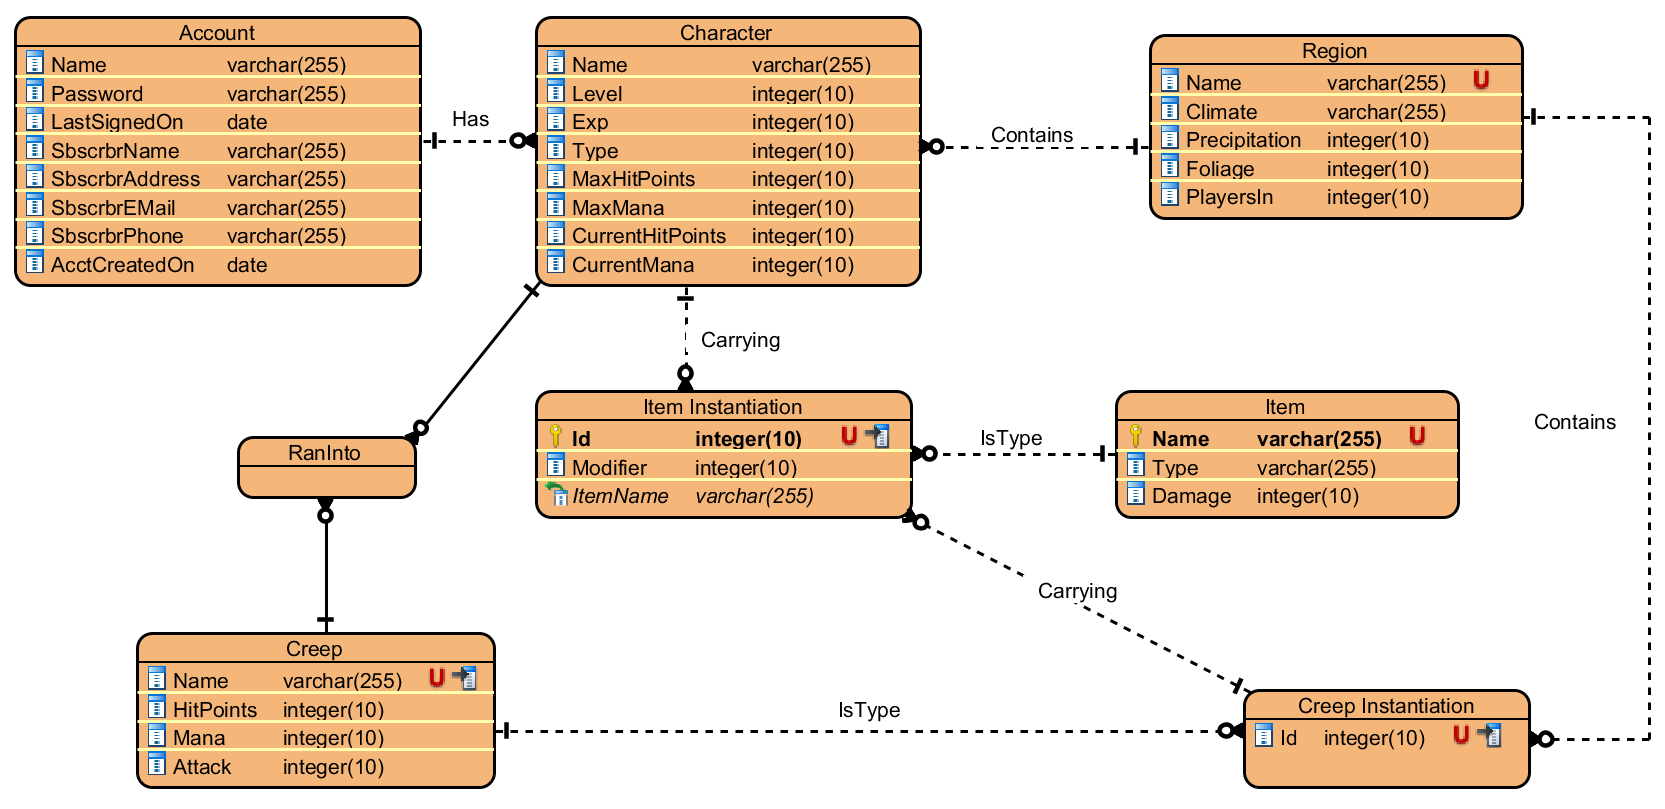
\includegraphics[width=\textwidth]{erCrowsFoot.png}
\end{center}

Нотация получила своё название за обозначение множественности связи (три разветвляющиеся линии на конце связи, похожие на птичью ногу). Её важное отличие от нотации Чена в том, что атрибуты в ней рисуются прямо внутри сущности, что делает диаграммы гораздо более компактными. Здесь тоже можно назначить один из атрибутов первичным ключом, задать ограничения уникальности и т.д., но детали нотации несколько различаются от инструмента к инструменту, поэтому не будем здесь на ней подробно останавливаться (благо такие диаграммы вы наверняка уже видели в контексте баз данных).

\subsection{Object-Role Modeling}

Object-Role Modeling (ORM) --- это ещё одна нотация для построения концептуальной модели предметной области и, в конечном итоге, схемы базы данных проектируемой системы. Она гораздо реже используется, чем ER-диаграммы, но считается довольно прогрессивной и хорошо подходящей именно для анализа. Нотация очень проста, в ней есть только сущности и связи, атрибутов нет. Зато связи более хитрые, они часто n-арные (в ER-диаграммах были возможны только бинарные связи) и могут быть соединены ограничениями. Вот пример такой диаграммы, описывающей сотрудников некоего университета:

\begin{center}
    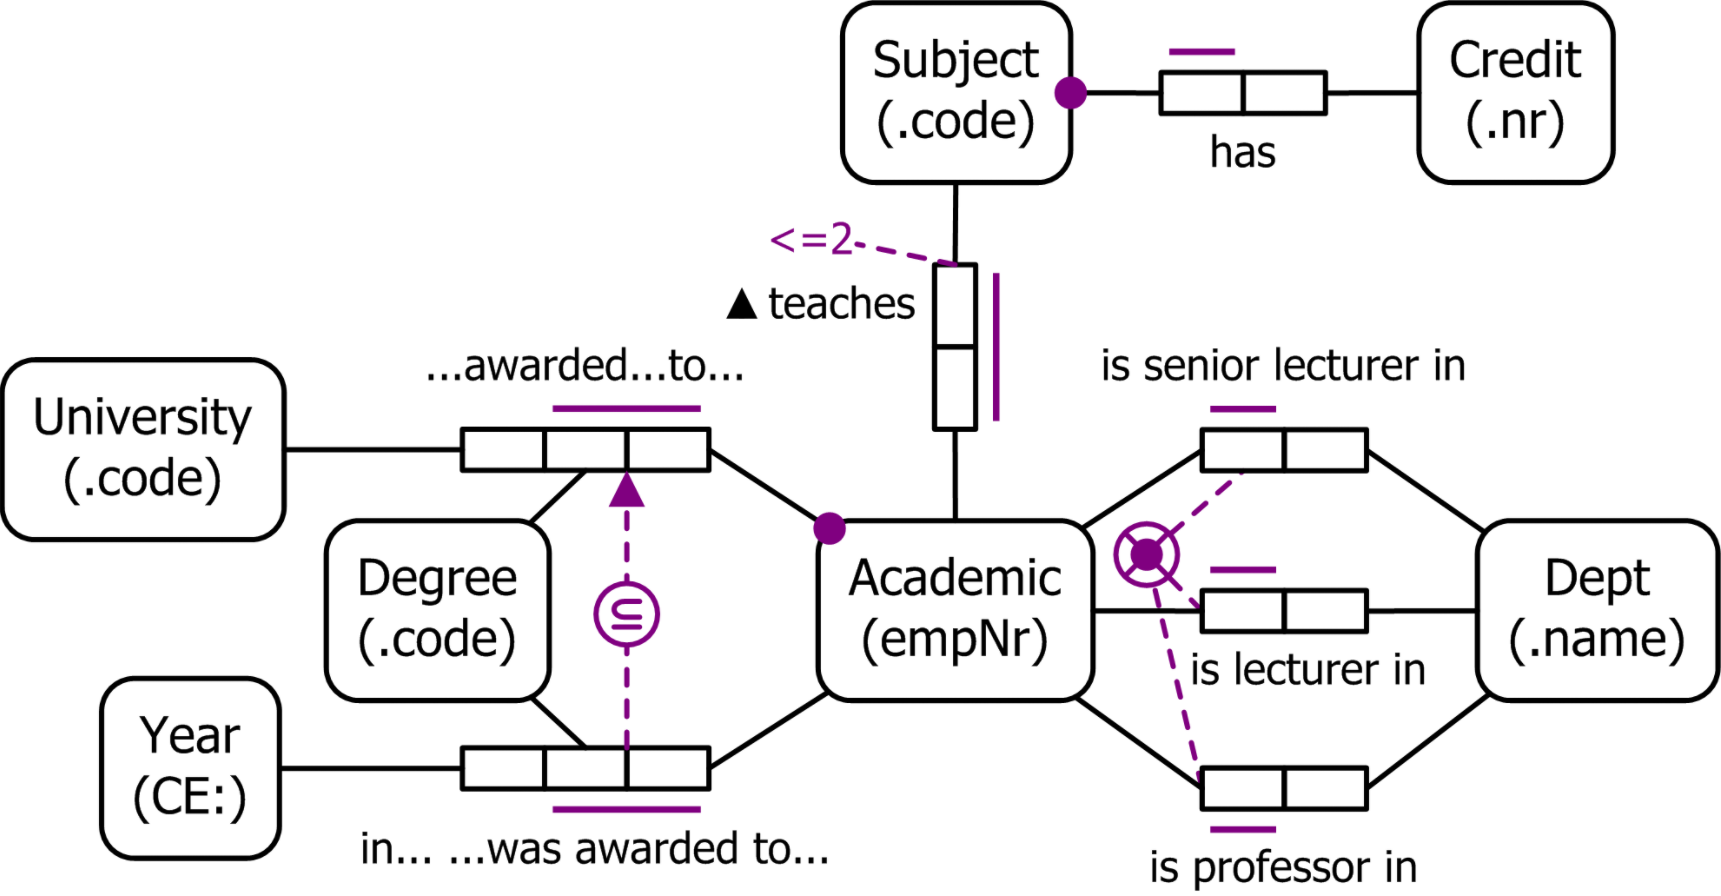
\includegraphics[width=0.8\textwidth]{orm.png}
    \attribution{http://www.orm.net}
\end{center}

Сущность имеет схему идентификации (её единственный атрибут --- признак, по которому её можно отличить от других), это то, что пишется в скобках. Связи играют роль таблиц в реляционной модели --- каждая связь представляет собой кортеж из нескольких сущностей, сущности играют в связи \textit{роли}, обозначаемые прямоугольниками посреди связи. Над связью пишется вариант прочтения, например, <<Университет такой-то присудил степень такую-то человеку такому-то>>. Это нужно прежде всего для лёгкости чтения диаграммы неспециалистами, и чтобы аналитик мог проверить естественным языком, что он делает что-то разумное. Горизонтальные и вертикальные полосы над ролями показывают, какие сочетания сущностей в данной связи должны быть уникальны. Роли могут быть связаны ограничениями, например, <<исключающего или>>: препод может быть либо преподавателем, либо старшим преподавателем, либо профессором на факультете.

Такие диаграммы используются реже ER-диаграмм в силу того, что для сколько-нибудь больших предметных областей ORM-диаграммы существенно больше по размеру, чем ER (каждый атрибут всё-таки надо моделировать как сущность). Зато такие диаграммы более устойчивы к изменениям в предметной области или нашего её понимания --- если мы в ER-диаграмме что-то сделали атрибутом, а потом оказалось, что у этого чего-то тоже есть атрибуты, нам придётся полдиаграммы переделывать (потому что атрибут атрибуты иметь не может). В ORM же просто добавляем новую связь с новой сущностью, и всё. Поэтому ORM-диаграммы считаются удобнее на первых этапах анализа, когда наших знаний ещё недостаточно, чтобы понять, кто сущность, а кто атрибут.

Обратите внимание, что ORM в программировании чаще используется в другом смысле --- Object-Relational Mapping. Это библиотеки (точнее, обычно целые технологии), которые представляют содержимое реляционной базы как набор настоящих объектно-ориентированных объектов и наоборот, так что при написании программы мы просто как обычно манипулируем объектами, меняем их свойства, создаём и удаляем и т.д., а ORM-система транслирует все наши действия в запросы к БД, беря на себя все проблемы с тем, что объектно-ориентированное программирование с реляционной моделью совсем не дружат. Например, в реляционной модели невозможно выразить наследование и даже отношение <<многие-ко-многим>>, так что ORM-системы нетривиальны. Так вот, в этом разделе речь шла не про то.

\end{document}
